\section{Acoustically-forced Transient Flame}\label{sec:oneDFlame}

The one-dimensional model of an acoustically-forced, freely-propagating premixed flame is now described. Similar constructions have been presented in prior work by the author and collaborators~\cite{Huang2022,Wentland2019}. The spatial domain is one-dimensional, spanning the length $x \in [0.0, \; 10]$ mm, subdivided into 1,024 cells of equal length. As with GEMS, a second-order Roe flux computes the inviscid fluxes, while gradients are computed by a central finite-difference stencil and limited by the face-oriented limiter of Barth and Jespersen.

The chemical system is composed of two fictitious species, a ``reactant'' species and a ``product'' species, having the calorically-perfect gas properties given in Table~\ref{tab:oneDFlameSpecs}. In this case, the fluid has a constant viscosity, unlike results in Section~\ref{sec:cavity} which computed viscosity via Sutherland's law. Note that the only difference between the two species is their enthalpy of formation. The reactant is converted to product by a single irreversible finite-rate reaction, governed by the Arrhenius parameters $A = 2.12 \times 10^{10}$ 1/s, $b = 0$, and $E_a = 2.025 \times 10^{8}$ kJ/mol.

\begin{table}
	\centering
	\begin{tabular}{ lllllll }
	\toprule
	Species & MW (g/mol) & $\cpSpec$ (kJ/kg-K) & $\refEnthSpec$ (kJ/kg) & $\dynViscSpec$ (kg/m-s) & $\prandtlSpec$ & $\schmidtSpec$   \\
	\midrule
	Reactant & 21.32 & 1.538 & -7,4320 & 7.35e-4 & 0.713 & 0.62 \\
	Product & 21.32 & 1.538 & -10,800 & 7.35e-4 & 0.713 & 0.62 \\
	\bottomrule
	\end{tabular}
	\caption{\label{tab:oneDFlameSpecs}Constant thermodynamic and transport properties of fictitious species.}
\end{table}

To begin, the solution is initialized with 100\% reactant at 300 K in the region $x \in [0.0, \; 0.02]$ mm, and the remainder of the domain is initialized with product at 2,400 K. The full domain is initialized with a pressure of 1 MPa and zero velocity. An approximate characteristic boundary condition is enforced at the outlet, and a fixed velocity is enforced at the inlet. Using BDF2 integration with a time step of 25 ns, the simulation is started with a velocity of 1 m/s at the inlet, which is manually adjusted until the flame is determined to be suitably ``stationary,'' balancing the bulk advection downstream with the reaction/diffusion upstream. At this point, 10 m/s is added to the velocity throughout the domain, and the primitive state appears as shown in Fig.~\ref{fig:flameIC}. This is the initial condition from which all further FOM simulations are computed. Further, for all further simulations (ROM or FOM), the inlet boundary condition is changed to an approximate characteristic boundary condition.

\begin{figure}
	\begin{minipage}{0.49\linewidth}
		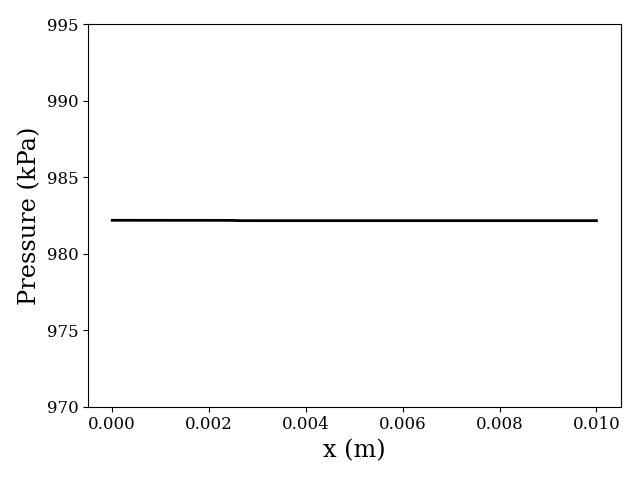
\includegraphics[width=0.99\linewidth]{Chapters/TransientFlame/Images/init_cond_pressure.png}
	\end{minipage}
	\begin{minipage}{0.49\linewidth}
		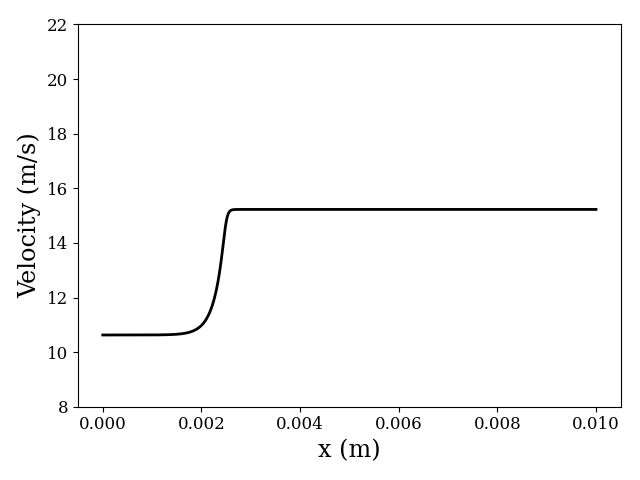
\includegraphics[width=0.99\linewidth]{Chapters/TransientFlame/Images/init_cond_vel.png}
	\end{minipage}

	\begin{minipage}{0.49\linewidth}
		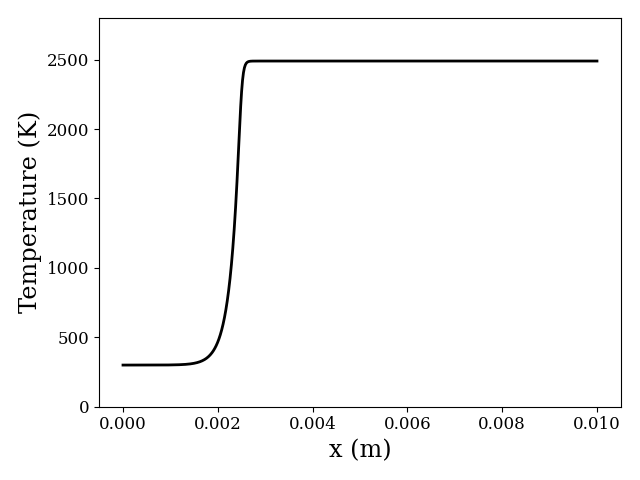
\includegraphics[width=0.99\linewidth]{Chapters/TransientFlame/Images/init_cond_temp.png}
	\end{minipage}
	\begin{minipage}{0.49\linewidth}
		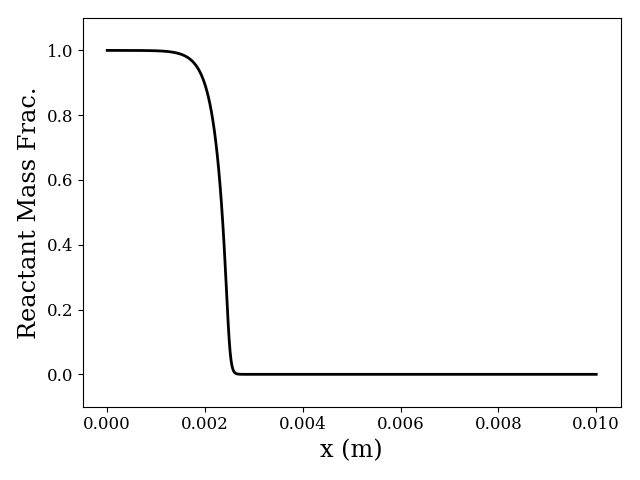
\includegraphics[width=0.99\linewidth]{Chapters/TransientFlame/Images/init_cond_mf.png}
	\end{minipage}
	\caption{\label{fig:flameIC}Initial condition for propagating flame FOM simulations.}
\end{figure}

To build a dataset of parametrically-varied simulations, an artificial pressure forcing is introduced to the outlet boundary condition. This forcing is computed as a sinusoidal perturbation about the outlet mean-flow pressure, of the form
%
\begin{equation}
	\pressureBack = \pressureMean \left[1 + A \; sin\left(2 \pi f \timeVar\right)\right]
\end{equation}
%
where $\pressureMean$ is the outlet mean-flow pressure (approximately 965 kPa in this case), $A$ is the percentage amplitude, and $f$ is the forcing frequency. For all cases, the amplitude is 1\%. A total of 21 FOM simulations are computed with different forcing frequencies $f$, ranging from 87.5 to 212.5 kHz at intervals of 6.26 kHz. Each simulation is allowed to run for 23,000 iterations, or 575 $\mu$s. Snapshots of the primitive state are collected at every 10 iterations, starting after 3,000 iterations ($\timeVar = 75 \mu$s). for a total of 2,000 snapshots per FOM simulation. The data are then split into nine training, three validation, and nine test sets. The first group will be explicitly used to train the data-driven models, the second will be used for neural network training to inform model generalizability during the learning process, and the third will be used to evaluate the predictive capabilities of the resulting models.

\begin{table}
	\centering
	\begin{tabular}{ lll }
	\toprule
	Training & Validation & Testing  \\
	\midrule
	100   & 118.75 & 87.5 \\
	112.5 & 156.25 & 93.75 \\
	125   & 193.75 & 106.25 \\
	137.5 &        & 131.25 \\
	150   &        & 143.75 \\
	162.5 &        & 168.75 \\
	175   &        & 181.25 \\
	187.5 &        & 206.25 \\
	200   &        & 212.5 \\
	\bottomrule
	\end{tabular}
	\caption{\label{tab:trainSplit}Training, validation, and testing dataset splits, by forcing frequency (in kHz).}
\end{table}

Examples of several relevant flow fields are given in Figs.~\ref{fig:flameFOMPress} and~\ref{fig:fig:flameFOMFlame}. Pressure snapshots for several different forcing frequencies are shown in Fig.~\ref{fig:flameFOMPress}, where it is clear that the acoustic behavior is significantly affected by the disparate sound speeds between the hot products and cold reactants, increasing the frequency and amplitude of the signal as it propagates upstream. Figure~\ref{fig:flameFOMFlame} shows two relevant indicators of the flame's propagation downstream, marked by a steep rise in temperature where cold reactant is converted to hot product, and the peak of maximum heat release indicates the precise location of this reaction. 

\begin{figure}
	\centering
	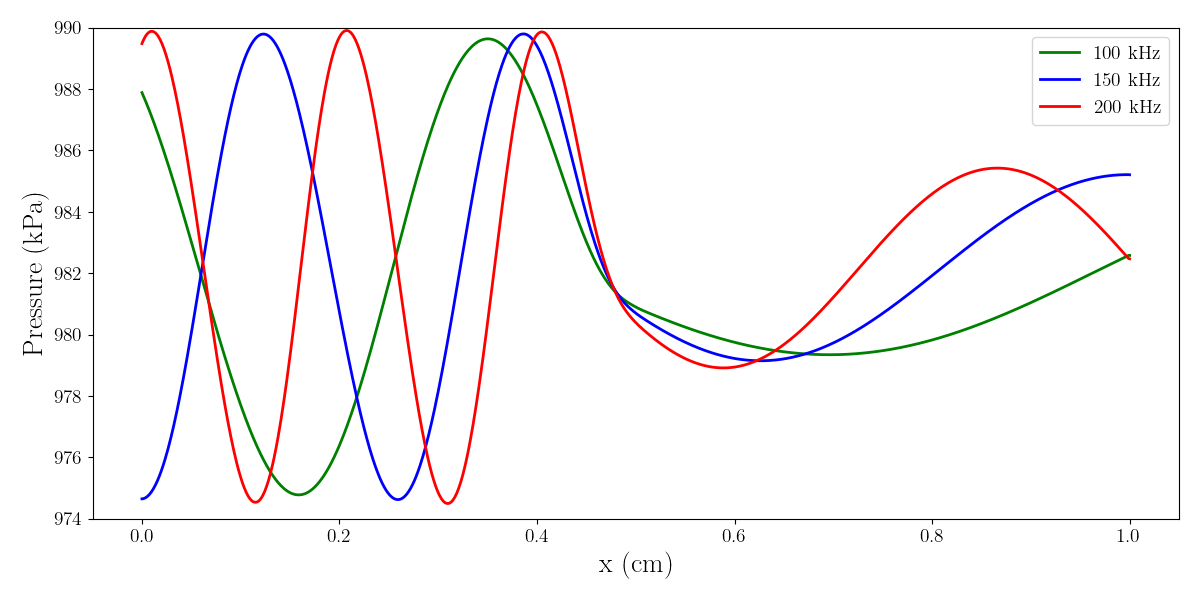
\includegraphics[width=0.9\linewidth]{Chapters/TransientFlame/Images/fom/fom_press_snaps.png}
	\caption{\label{fig:flameFOMPress}Forced pressure field examples, $f \in \{100, \; 150, \; 200\}$ kHz.}
\end{figure}

\begin{figure}
	\begin{minipage}{0.49\linewidth}
		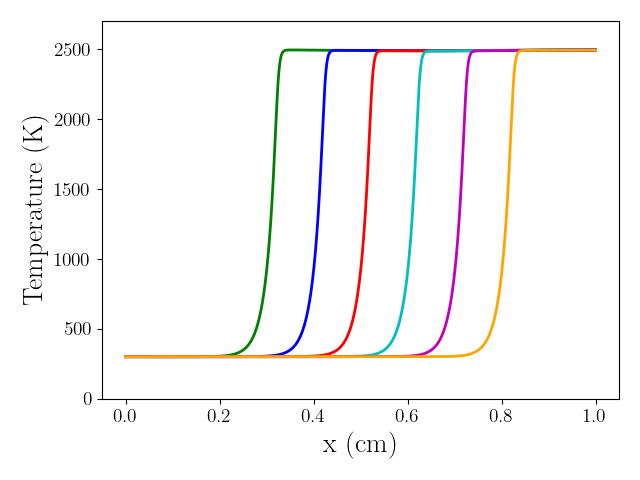
\includegraphics[width=0.99\linewidth]{Chapters/TransientFlame/Images/fom/fom_temp_snaps.png}
	\end{minipage}
	\begin{minipage}{0.49\linewidth}
		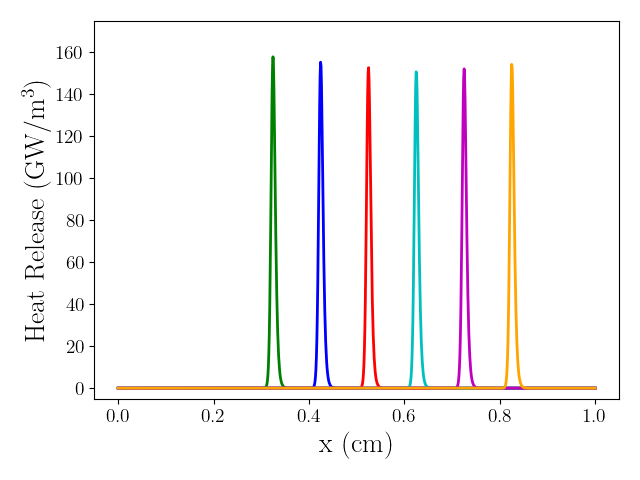
\includegraphics[width=0.99\linewidth]{Chapters/TransientFlame/Images/fom/fom_hr_snaps.png}
	\end{minipage}
	\caption{\label{fig:flameFOMFlame}Flame progression for data collection period $\timeVar \in [75, \; 575] \; \mu$s.}
\end{figure}

This case presents several interesting challenges for data-driven modeling and PROMs in particular. The system is characterized by three different spatio-temporal scales, namely those associated with the bulk advection, acoustics, and reaction. Traditional approaches to model reduction often struggle to accurately model phenomena such as sharp gradients, propagating waves, and highly non-linear multi-physics couplings. As will be shown shortly, classical methods (and even some novel machine learning approaches) generally fail to make accurate predictions.